\documentclass{article}
\usepackage{amsmath, amssymb, ctex, graphicx, color}
\usepackage[margin=1in]{geometry}
\usepackage{setspace} % 行距控制
\usepackage{array}
\usepackage{makecell}
\usepackage{booktabs}

\usepackage{algorithm}
\usepackage{algpseudocode}
\usepackage{xcolor}
% 把默认注释符号 ▷ 改成行尾 // 等宽紫色，并右对齐
\renewcommand{\algorithmiccomment}[1]{\hfill\texttt{\textcolor{violet}{// #1}}}
% 定义 Input / Output 关键字（默认是 Require / Ensure）
\algnewcommand\algorithmicinput{\textbf{Input:}}
\algnewcommand\algorithmicoutput{\textbf{Output:}}
\algnewcommand\Input{\item[\algorithmicinput]}
\algnewcommand\Output{\item[\algorithmicoutput]}

\usepackage{titling}\setlength{\droptitle}{-2cm} 
\title{Ch8. Backpropagation \hfill 第8章 反向传播 \\ 
Section 8.2. Automatic Differentiation \hfill 第8.2节 自动微分法 \\ 
8.2.1 Forward-mode AD \hfill 8.2.1. 前向模式自动微分}
\author{《深度学习基础》课程小组}
% \date{}
 
\begin{document}
\maketitle
% \tableofcontents

\setlength{\parindent}{0pt} % 取消首行缩进
\setlength{\parskip}{1.5em} % 设置段落之间的距离

\noindent\rule{\linewidth}{0.4pt}

\section{P1}

In forward-mode automatic differentiation, we augment each intermediate variable $z_i$, known as a `primal' variable, involved in the evaluation of a function, such as the error function of a neural network, with an additional variable representing the value of some derivative of that variable, which we can denote $\dot{z}_i$, known as a `tangent' variable. 

The tangent variables and their associated code are generated automatically by the software environment. 

Instead of simply doing forward propagation to compute $\{z_i\}$, the code now propagates tuples $(z_i, \dot{z}_i)$ so that variables and derivatives are evaluated in parallel. 

The original function is generally defined in terms of elementary operators consisting of arithmetic operations and negation as well as transcendental functions such as exponential, logarithm, and trigonometric functions, all of which have simple formulae for their derivatives. 

Using these derivatives in combination with the chain rule of calculus allows the code used to evaluate gradients to be constructed automatically.

% 翻译这段话。然后补充几句话，解读这段话里的重点难点。请输出为latex代码，以便于复制修改排版。

{\color{red}
翻译：% {前向模式自动微分}

在前向模式自动微分中，我们为每一个参与函数求值的中间变量 $z_i$（称为\textbf{主变量}（primal variable））附加一个额外的变量，用以表示该变量的某种导数值，记为 $\dot{z}_i$，称为\textbf{切线变量}（tangent variable）。这里的函数可以是神经网络的误差函数等。

切线变量及其相关代码由软件环境自动生成。

代码不再仅仅进行前向传播以计算 $\{z_i\}$，而是传播元组 $(z_i, \dot{z}_i)$，使得变量值与导数值被\textbf{并行}计算。

原始函数通常由\textbf{基本算子}（elementary operators）定义，包括算术运算、取反，以及指数、对数、三角函数等超越函数——这些运算的导数公式都是已知的、形式简单的。

将这些导数公式与微积分中的\textbf{链式法则}结合使用，便可自动构建用于计算梯度的代码。
}

{\color{blue}
重点与难点解读：

\paragraph{1. ``增强''（augment）的思想}
这段话的核心思想是\textbf{变量增强}：对计算图中的每个中间变量 $z_i$，都"绑定"一个伴随变量 $\dot{z}_i$。这种增强不是数学上的新定义，而是一种\textbf{编程实现策略}——它使得每次计算 $z_i$ 时，其导数 $\dot{z}_i$ 也能被同步、自动地计算出来，无需手动推导或编写求导代码。

\paragraph{2. 元组传播 $(z_i, \dot{z}_i)$ 的含义}
前向传播原本只传递数值 $z_i$；增强后则传递\textbf{二元组}。这意味着每经过一个基本运算（如乘法 $v_3 = v_1 \cdot v_2$），程序不仅计算 $v_3$ 的值，还利用乘积法则同时计算 $\dot{v}_3 = \dot{v}_1 v_2 + v_1 \dot{v}_2$。整个过程就像一条"双轨流水线"，一轨算函数值，一轨算导数值，二者同步前进。

\paragraph{3. 为什么只需基本算子？}
自动微分的关键假设是：任何复杂函数最终都可以\textbf{分解}为有限个基本算子（加、减、乘、除、$\exp$、$\log$、$\sin$ 等）的组合。只要每个基本算子的导数公式已知且简单，链式法则就能将它们逐层"串联"起来，自动得到整个复合函数的导数。这正是自动微分区别于\textbf{符号微分}（试图对整个表达式求闭合形式导数）和\textbf{数值微分}（用有限差分近似）的本质所在。

\paragraph{4. 前向模式的计算代价}
值得注意的是，一次前向传播只能计算函数对\textbf{一个}输入变量的导数（即 $\dot{z}_i = \partial z_i / \partial x_j$，其中 $x_j$ 是事先选定的那个输入）。如果函数有 $D$ 个输入，就需要 $D$ 次前向传播才能获得完整梯度。当 $D$ 很大时（如神经网络的数百万参数），前向模式效率极低，这正是后文引入\textbf{反向模式自动微分}（reverse-mode AD，即反向传播算法）的动机。
}

\noindent\rule{\linewidth}{0.4pt}

\section{P2}

As an example, consider the following function, which has two input variables:
\begin{equation}
f(x_1, x_2) = x_1 x_2 + \exp(x_1 x_2) - \sin(x_2).
\tag{8.49}
\end{equation}
When implemented in software, the code consists of a sequence of operations that can be expressed as an \emph{evaluation trace} of the underlying elementary operations. 

This trace can be visualized in the form of a graph, as shown in Figure~8.4. 

Figure 8.4 Caption: Evaluation trace diagram showing the steps involved in the numerical evaluation
of the function (8.49) using the primal equations (8.50) to (8.56).

\begin{figure}[htbp]
    \centering
    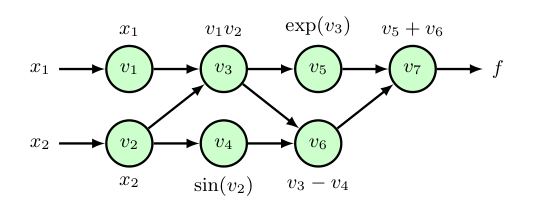
\includegraphics[width=0.5\textwidth]{figure-8-4.png}
    \caption{图8-4：前向自动微分的例子}
    % \label{}
\end{figure}

Here we have defined the following primal variables
\begin{align}
v_1 &= x_1 \tag{8.50} \\
v_2 &= x_2 \tag{8.51} \\
v_3 &= v_1 v_2 \tag{8.52} \\
v_4 &= \sin(v_2) \tag{8.53} \\
v_5 &= \exp(v_3) \tag{8.54} \\
v_6 &= v_3 - v_4 \tag{8.55} \\
v_7 &= v_5 + v_6. 
\tag{8.56}
\end{align}

Now suppose we wish to evaluate the derivative $\partial f / \partial x_1$. 

We define the tangent variables by $\dot{v}_i = \partial v_i / \partial x_1$. 

Expressions for evaluating these can be constructed automatically using the chain rule of calculus:
\begin{equation}
\dot{v}_i = \frac{\partial v_i}{\partial x_1} 
= \sum_{j \in \mathrm{pa}(i)} \frac{\partial v_j}{\partial x_1} \frac{\partial v_i}{\partial v_j}
= \sum_{j \in \mathrm{pa}(i)} \dot{v}_j \frac{\partial v_i}{\partial v_j}.
\tag{8.57}
\end{equation}
where $\mathrm{pa}(i)$ denotes the set of \emph{parents} of the node $i$ in the evaluation trace diagram, that is the set of variables with arrows pointing to node $i$. 

For example, in Figure~8.4 the parents of node $v_3$ are nodes $v_1$ and $v_2$. 

Applying (8.57) to the evaluation trace equations (8.50) to (8.56), we obtain the following evaluation trace equations for the tangent variables
\begin{align}
\dot{v}_1 &= 1 \tag{8.58} \\
\dot{v}_2 &= 0 \tag{8.59} \\
\dot{v}_3 &= \dot{v}_1 v_2 + v_1 \dot{v_2} \tag{8.60} \\
\dot{v}_4 &= \dot{v}_2 \cos(v_2) \tag{8.61} \\
\dot{v}_5 &= \dot{v}_3 \exp(v_3) \tag{8.62} \\
\dot{v}_6 &= \dot{v}_3 - \dot{v}_4 \tag{8.63} \\
\dot{v}_7 &= \dot{v}_5 + \dot{v}_6. 
\tag{8.64}
\end{align}

% 翻译这段话。然后补充几句话，解读这段话里的重点难点。请输出为latex代码，以便于复制修改排版。

{\color{red}
翻译：%{前向模式自动微分示例（翻译与解读）}

作为一个例子，考虑以下具有两个输入变量的函数：
\begin{equation}
f(x_1, x_2) = x_1 x_2 + \exp(x_1 x_2) - \sin(x_2).
\tag{8.49}
\end{equation}
在软件中实现时，代码由一系列操作组成，这些操作可以表示为底层基本运算的\emph{求值轨迹}（evaluation trace）。

该轨迹可以用图的形式可视化，如图~8.4 所示。

这里我们定义了以下主变量：
\begin{align}
v_1 &= x_1 \tag{8.50} \\
v_2 &= x_2 \tag{8.51} \\
v_3 &= v_1 v_2 \tag{8.52} \\
v_4 &= \sin(v_2) \tag{8.53} \\
v_5 &= \exp(v_3) \tag{8.54} \\
v_6 &= v_3 - v_4 \tag{8.55} \\
v_7 &= v_5 + v_6. 
\tag{8.56}
\end{align}

现在假设我们希望计算导数 $\partial f / \partial x_1$。

我们通过 $\dot{v}_i = \partial v_i / \partial x_1$ 来定义切线变量。

利用微积分中的链式法则，可以自动构建用于计算这些切线变量的表达式：
\begin{equation}
\dot{v}_i = \frac{\partial v_i}{\partial x_1} 
= \sum_{j \in \mathrm{pa}(i)} \frac{\partial v_j}{\partial x_1} \frac{\partial v_i}{\partial v_j}
= \sum_{j \in \mathrm{pa}(i)} \dot{v}_j \frac{\partial v_i}{\partial v_j},
\tag{8.57}
\end{equation}
其中 $\mathrm{pa}(i)$ 表示求值轨迹图中节点 $i$ 的\emph{父节点}集合，即所有有箭头指向节点 $i$ 的变量集合。

例如，在图~8.4 中，节点 $v_3$ 的父节点是节点 $v_1$ 和 $v_2$。

将式 (8.57) 应用于求值轨迹方程 (8.50) 至 (8.56)，我们可以得到以下切线变量的求值轨迹方程：
\begin{align}
\dot{v}_1 &= 1 \tag{8.58} \\
\dot{v}_2 &= 0 \tag{8.59} \\
\dot{v}_3 &= \dot{v}_1 v_2 + v_1 \dot{v_2} \tag{8.60} \\
\dot{v}_4 &= \dot{v}_2 \cos(v_2) \tag{8.61} \\
\dot{v}_5 &= \dot{v}_3 \exp(v_3) \tag{8.62} \\
\dot{v}_6 &= \dot{v}_3 - \dot{v}_4 \tag{8.63} \\
\dot{v}_7 &= \dot{v}_5 + \dot{v}_6. 
\tag{8.64}
\end{align}

}

{\color{blue}
重点与难点解读：

\paragraph{1. 求值轨迹（Evaluation Trace）的本质}
求值轨迹是将一个复杂函数\textbf{分解为基本运算序列}的具体体现。它不仅是可视化的计算图，更是自动微分的\textbf{执行蓝图}。每一个中间变量 $v_i$ 对应一个计算节点，而节点之间的边代表了数据依赖关系。理解这一点是掌握自动微分的基础——我们不再把函数看作一个整体，而是看作一张可遍历的有向无环图（DAG）。

\paragraph{2. 链式法则的局部化应用}
公式 (8.57) 是整段的核心。它将全局的链式法则$\frac{\partial v_i}{\partial x_1}$转化为仅依赖\textbf{直接父节点}的局部求和。这意味着每个节点的切线变量$\dot{v}_i$只需知道其父节点的切线值$\dot{v}_j$和局部偏导$\frac{\partial v_i}{\partial v_j}$即可算出。这种\textbf{局部性}正是自动微分能够"自动"进行的关键：无需推导整个函数的解析导数，只需逐节点应用已知的局部导数规则。

\paragraph{3. 初始条件的设定逻辑}
注意式 (8.58) 和 (8.59)：$\dot{v}_1 = 1$、$\dot{v}_2 = 0$。这是因为我们求的是对$x_1$的偏导，所以只有$x_1$对应的切线初值为1，其余输入变量的切线初值均为0。这体现了前向模式的一个关键特性：\textbf{一次前向传播只能计算对一个特定输入的导数}。若要计算$\partial f/\partial x_2$，则需重新初始化$\dot{v}_1=0, \dot{v}_2=1$并再次执行整个轨迹。

}

\noindent\rule{\linewidth}{0.4pt}

\section{P3}

We can summarize code to implement the evaluation of the primal variables, given by (8.50) to (8.56). 

The associated equations and corresponding code for evaluating the tangent variables (8.58) to (8.64) are generated automatically. 

To evaluate the derivative $\partial f / \partial x_1$, we input specific values of $x_1$ and $x_2$ and the code then executes the primal and tangent passes, numerically evaluating the tuples $(v_i, \dot{v}_i)$ in sequence until we obtain $\dot{v}_7$, which is the required derivative.

翻译这段话。然后补充几句话，解读这段话里的重点难点。请输出为latex代码，以便于复制修改排版。

{\color{red}
翻译：%{前向模式自动微分的代码实现（翻译与解读）}

我们可以编写代码来实现由式 (8.50) 至 (8.56) 给出的主变量求值过程。

用于计算切线变量的相关方程 (8.58) 至 (8.64) 及其对应代码，则由系统自动生成。

为了计算导数 $\partial f / \partial x_1$，我们输入 $x_1$ 和 $x_2$ 的具体数值，随后代码依次执行主变量传递（primal pass）与切线变量传递（tangent pass），按顺序对元组 $(v_i, \dot{v}_i)$ 进行数值计算，直至得到 $\dot{v}_7$，该值即为所求的导数。
}

{\color{blue}
重点与难点解读：

\paragraph{1. “自动生成”的工程含义}
这段话揭示了自动微分框架（如 PyTorch、JAX）的核心工作机制：用户只需定义主变量的计算逻辑（即前向传播代码），而切线变量的计算代码完全由编译器或解释器通过源码变换（source transformation）或运算符重载（operator overloading）自动生成。这从根本上将算法开发者从繁琐且易错的手动求导中解放出来，是深度学习框架得以普及的关键工程基础。

\paragraph{2. 元组 $(v_i, \dot{v}_i)$ 的同步计算}
文中强调“按顺序对元组进行数值计算”，这表明在前向模式中，函数值 $v_i$ 与其导数 $\dot{v}_i$ 是在同一次遍历中被同时计算的，而非先算完所有 $v_i$ 再回头算 $\dot{v}_i$。这种同步性保证了每个节点在计算切线时，其依赖的主变量值已经就绪，避免了额外的存储开销和重复计算，但也意味着内存中必须同时保存值和导数两份数据。

\paragraph{3. 数值计算 vs 符号推导}
需特别注意，自动微分执行的是“数值计算”而非“符号推导”。给定具体的 $x_1, x_2$ 数值后，$(v_i, \dot{v}_i)$ 全程以浮点数形式传播，不会生成任何解析表达式。这意味着自动微分的结果是特定输入点处的精确导数值（精度等同于机器浮点运算），既不同于符号微分的闭合公式，也不同于有限差分的近似估计。理解这一区别对于正确调试梯度问题和优化计算性能至关重要。
}

\noindent\rule{\linewidth}{0.4pt}

\section{P4}

Now consider an example with two outputs $f_1(x_1, x_2)$ and $f_2(x_1, x_2)$ where $f_1(x_1, x_2)$ is defined by (8.49) and
\begin{equation}
f_2(x_1, x_2) = (x_1 x_2 - \sin(x_2)) \exp(x_1 x_2)
\tag{8.65}
\end{equation}
as illustrated by the evaluation trace diagram in Figure~8.5. 

Figure 8.5 Caption: Extension of the example shown in Figure 8.4 to a function with two outputs $f_1$ and
$f_2$.

\begin{figure}[htbp]
    \centering
    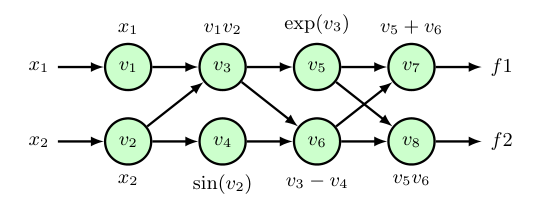
\includegraphics[width=0.5\textwidth]{figure-8-5.png}
    \caption{图8-5：前向自动微分的又一个例子}
    % \label{}
\end{figure}

We see that this involves only a small extension to the evaluation equations for the primal and tangent variables, and so both $\partial f_1 / \partial x_1$ and $\partial f_2 / \partial x_1$ can be evaluated together in a single forward pass. 

The downside, however, is that if we wish to evaluate derivatives with respect to a different input variable $x_2$ then we have to run a separate forward pass.

In general, if we have a function with $D$ inputs and $K$ outputs, then a single pass of forward-mode automatic differentiation produces a single column of the $K \times D$ Jacobian matrix:
\begin{equation}
\mathbf{J} =
\begin{bmatrix}
\displaystyle \frac{\partial f_1}{\partial x_1} & \cdots & \displaystyle \frac{\partial f_1}{\partial x_D} \\
\vdots & \ddots & \vdots \\
\displaystyle \frac{\partial f_K}{\partial x_1} & \cdots & \displaystyle \frac{\partial f_K}{\partial x_D}
\end{bmatrix}.
\tag{8.66}
\end{equation}

To compute column $j$ of the Jacobian, we need to initialize the forward pass of the tangent equations by setting $\dot{x}_j = 1$ and $\dot{x}_i = 0$ for $i \ne j$. 

We can write this in vector form as $\dot{\mathbf{x}} = \mathbf{e}_j$, where $\mathbf{e}_j$ is the $j$th unit vector. 

To compute the full Jacobian matrix we need $D$ forward-mode passes. 

However, if we wish to evaluate the product of the Jacobian with a vector $\mathbf{r} = (r_1, \dots, r_D)^{\mathsf{T}}$:
\begin{equation}
\mathbf{J} = 
\begin{bmatrix}
\displaystyle \frac{\partial f_1}{\partial x_1} & \cdots & \displaystyle \frac{\partial f_1}{\partial x_D} \\
\vdots & \ddots & \vdots \\
\displaystyle \frac{\partial f_K}{\partial x_1} & \cdots & \displaystyle \frac{\partial f_K}{\partial x_D}
\end{bmatrix}
\begin{bmatrix}
r_1 \\ \vdots \\ r_D
\end{bmatrix},
\tag{8.67}
\end{equation}
then this can be done in a single forward pass by setting $\dot{\mathbf{x}} = \mathbf{r}$.

% 翻译这段话。然后补充几句话，解读这段话里的重点难点。请输出为latex代码，以便于复制修改排版。


{\color{red}
翻译：%{多输出函数与前向模式的雅可比矩阵（翻译与解读）}

现在考虑一个具有两个输出 $f_1(x_1, x_2)$ 和 $f_2(x_1, x_2)$ 的例子，其中 $f_1(x_1, x_2)$ 由式 (8.49) 定义，而
\begin{equation}
f_2(x_1, x_2) = (x_1 x_2 - \sin(x_2)) \exp(x_1 x_2)
\tag{8.65}
\end{equation}
如图~8.5 的求值轨迹图所示。

我们可以看到，这仅仅需要对主变量和切线变量的求值方程做少量扩展，因此 $\partial f_1 / \partial x_1$ 和 $\partial f_2 / \partial x_1$ 可以在\textbf{同一次前向传播}中一起计算出来。

然而，其缺点在于：如果我们希望计算关于另一个输入变量 $x_2$ 的导数，就必须\textbf{再单独执行一次}前向传播。

一般地，如果我们有一个具有 $D$ 个输入和 $K$ 个输出的函数，那么前向模式自动微分的\textbf{一次传播}可以产生 $K \times D$ 雅可比矩阵的\textbf{一列}：
\begin{equation}
\mathbf{J} =
\begin{bmatrix}
\displaystyle \frac{\partial f_1}{\partial x_1} & \cdots & \displaystyle \frac{\partial f_1}{\partial x_D} \\
\vdots & \ddots & \vdots \\
\displaystyle \frac{\partial f_K}{\partial x_1} & \cdots & \displaystyle \frac{\partial f_K}{\partial x_D}
\end{bmatrix}.
\tag{8.66}
\end{equation}

为了计算雅可比矩阵的第 $j$ 列，我们需要通过设置 $\dot{x}_j = 1$ 且当 $i \ne j$ 时 $\dot{x}_i = 0$ 来初始化切线方程的前向传播。

我们可以将其写成向量形式 $\dot{\mathbf{x}} = \mathbf{e}_j$，其中 $\mathbf{e}_j$ 是第 $j$ 个单位向量。

为了计算完整的雅可比矩阵，我们需要 $D$ 次前向模式传播。

然而，如果我们希望计算雅可比矩阵与向量 $\mathbf{r} = (r_1, \dots, r_D)^{\mathsf{T}}$ 的乘积：
\begin{equation}
\mathbf{J}\mathbf{r} = 
\begin{bmatrix}
\displaystyle \frac{\partial f_1}{\partial x_1} & \cdots & \displaystyle \frac{\partial f_1}{\partial x_D} \\
\vdots & \ddots & \vdots \\
\displaystyle \frac{\partial f_K}{\partial x_1} & \cdots & \displaystyle \frac{\partial f_K}{\partial x_D}
\end{bmatrix}
\begin{bmatrix}
r_1 \\ \vdots \\ r_D
\end{bmatrix},
\tag{8.67}
\end{equation}
那么只需通过设置 $\dot{\mathbf{x}} = \mathbf{r}$，即可在\textbf{一次前向传播}中完成。
}

{\color{blue}
重点与难点解读：

\paragraph{1. 多输出"免费"扩展的优势}
增加输出数量几乎不增加额外计算代价。这是因为多个输出共享大量中间计算节点（如 $v_3 = x_1 x_2$ 同时被 $f_1$ 和 $f_2$ 使用），切线变量沿着同一张计算图向前传播，到达不同的输出节点时自然给出各自的导数值。这种\textbf{计算复用}是前向模式在 $K \gg D$（输出远多于输入）场景下高效的原因。

\paragraph{2. 雅可比矩阵的列视角}
这段话从矩阵角度清晰地揭示了前向模式的本质：每次传播通过设定不同的种子向量 $\mathbf{e}_j$，计算出雅可比矩阵的\textbf{一整列} $\left(\frac{\partial f_1}{\partial x_j}, \dots, \frac{\partial f_K}{\partial x_j}\right)^{\mathsf{T}}$。要获得完整的 $K \times D$ 雅可比矩阵，需要 $D$ 次传播。这一分析框架是理解后续反向模式（每次传播计算雅可比矩阵的\textbf{一整行}）的对照基础。

\paragraph{3. $D$ 次传播的代价瓶颈}
对于深度神经网络，输入维度 $D$（即参数量）通常在百万到十亿级别，而输出 $K$ 通常只有 1 个（标量损失函数）。这意味着前向模式需要 $D$ 次完整的前向传播才能算出梯度，而反向模式只需 $K=1$ 次反向传播。这一巨大的效率差异（$D$ 次 vs $1$ 次）正是\textbf{反向传播算法}（即反向模式自动微分）成为深度学习标准训练方法的根本原因。

\paragraph{4. 雅可比向量积（JVP）的实用价值}
式 (8.67) 展示了一个重要技巧：通过设置 $\dot{\mathbf{x}} = \mathbf{r}$（而非单位向量），一次前向传播即可计算雅可比向量积（Jacobian-Vector Product, JVP）$\mathbf{J}\mathbf{r}$。这在高阶优化（如 Hessian-free 优化）、信赖域方法以及某些需要方向导数的场景中非常有用，因为它避免了显式构造完整的雅可比矩阵，直接获得所需的投影结果，显著降低了计算和存储成本。

}

\noindent\rule{\linewidth}{0.4pt}

\section{P5}

We see that forward-mode automatic differentiation can evaluate the full $K \times D$ Jacobian matrix of derivatives using $D$ forward passes. 

This is very efficient for networks with a few inputs and many outputs, such that $K \gg D$. 

However, we often operate in a regime where we have just one function, namely the error function used for training, and large numbers of variables that we want to differentiate with respect to, comprising the weights and biases in the network, of which there may be millions or billions. 

In such situations, forward-mode automatic differentiation is extremely inefficient. 

We therefore turn to an alternative version of automatic differentiation based on the backwards flow of derivative data through the evaluation trace graph.

% 翻译这段话。然后补充几句话，解读这段话里的重点难点。请输出为latex代码，以便于复制修改排版。

{\color{red}
翻译：%{前向模式的局限性与反向模式的引入（翻译与解读）}

我们可以看到，前向模式自动微分能够通过 $D$ 次前向传播来计算完整的 $K \times D$ 雅可比导数矩阵。

对于输入少而输出多的网络（即满足 $K \gg D$），这种方法非常高效。

然而，在实际应用中，我们通常面对的是另一种情形：只有一个目标函数（即用于训练的损失函数），但却需要对大量变量（即网络中的权重和偏置）求导，这些变量的数量可能达到数百万甚至数十亿。

在这种情况下，前向模式自动微分的效率极其低下。

因此，我们转向自动微分的另一种形式，它基于导数数据在求值轨迹图中的\textbf{反向流动}。
}

{\color{blue}
重点与难点解读：

\paragraph{1. 计算复杂度的不对称性}
这段话的核心在于揭示了自动微分两种模式的\textbf{计算复杂度对偶性}：前向模式的代价正比于输入维度 $D$，反向模式的代价正比于输出维度 $K$。当 $K \ll D$ 时（如神经网络的标量损失对百万参数求导），反向模式只需常数级次数的反向传播即可获得完整梯度，相比前向模式获得了 $O(D)$ 倍的加速。这种不对称性是选择算法的根本依据。

\paragraph{2. ``单个误差函数''的关键假设}
文中强调``only one function, namely the error function''，这并非偶然。深度学习之所以能高效训练，正是因为我们将所有优化目标\textbf{压缩为一个标量损失}。如果任务要求同时输出每个样本对每个参数的独立导数（即完整雅可比矩阵），反向模式的优势将不复存在。理解这一前提有助于明白为何多任务学习、辅助损失等设计仍倾向于最终合并为单一标量进行反向传播。

\paragraph{3. ``反向流动''的直觉理解}
``Backwards flow of derivative data''是反向传播算法的精髓。与前向模式中切线变量 $\dot{v}_i$ 随计算图正向传播不同，反向模式定义伴随变量（adjoint）$\bar{v}_i = \partial f / \partial v_i$，从输出节点开始，沿计算图的边\textbf{逆方向}逐层累积梯度。这一过程本质上是链式法则的\textbf{从右到左}应用，它使得每个中间节点的梯度贡献只被计算一次并被所有下游路径共享，从而避免了前向模式中因重复遍历导致的冗余计算。

\paragraph{4. 工程实践中的隐含权衡}
虽然反向模式在计算上占优，但它需要在前向传播时\textbf{存储所有中间激活值}以供反向传播使用，这带来了显著的内存开销。相比之下，前向模式无需额外存储，内存占用与单次前向传播相当。因此，在内存受限或需要实时计算方向导数（如JVP）的场景中，前向模式仍有其不可替代的价值。现代框架（如JAX）同时支持两种模式，正是为了在不同约束下灵活选择最优策略。
}

\end{document}
